% -*- mode: TeX -*-
% -*- coding: utf-8 -*-


% \RequirePackage[l2tabu, orthodox]{nag}
% \documentclass[runningheads,a4paper]{utils/llncs}

% \usepackage[american]{babel}
% \usepackage{graphicx}
% \usepackage{tikz}
% \usepackage{mdframed}
% %extended enumerate, such as \begin{compactenum}
% \usepackage{paralist}
%
% %put figures inside a text
% %\usepackage{picins}
% %use
% %\piccaptioninside
% %\piccaption{...}
% %\parpic[r]{\includegraphics ...}
% %Text...
%
% %Sorts the citations in the brackets
% %\usepackage{cite}
%
% %for easy quotations: \enquote{text}
% \usepackage{csquotes}
%
% \usepackage[T1]{fontenc}
%
% %enable margin kerning
% \usepackage{microtype}
%
% %better font, similar to the default springer font
% \usepackage[%
% rm={oldstyle=false,proportional=true},%
% sf={oldstyle=false,proportional=true},%
% tt={oldstyle=false,proportional=true,variable=true},%
% qt=false%
% ]{cfr-lm}
% %
% %if more space is needed, exchange cfr-lm by mathptmx
% %\usepackage{mathptmx}
%
% \usepackage{acro}
% % *** capitalisation config for acronyms ***
% \usepackage{mfirstuc}
% \acsetup{
%     page-ref    = paren,% Seitennummer in Klammern
%     extra-style = comma,% extra-Informationen mit Komma anhängen
%     only-used   = false,% für das Beispiel auch die nicht verwendeten in die Liste aufnehmen
%     sort        = true, % Liste sortieren
%     uc-cmd      = \capitalisewords
% }
% % -*- mode: TeX -*-
% -*- coding: utf-8 -*-


\DeclareAcronym{abc4trust}{
	short        = ABC4Trust,
	long         = attribute-Based credentials for trust
}

\DeclareAcronym{cbis}{
    short           = CBIS,
    short-plural    = 's,
    long            = computer-based information system
}

\DeclareAcronym{cc}{
    short       = CC,
    long        = creative commons
}

\DeclareAcronym{cern}{
    short       = CERN,
    long        = Conseil Europ{\'e}en pour la Recherche Nucl{\'e}aire,
    foreign     = European Organization for Nuclear Research,
    foreign-lang = english
}

\DeclareAcronym{cscw}{
	short        = CSCW,
	long         = computer-Supported collaborative work
}

\DeclareAcronym{cscl}{
	short        = CSCL,
	long         = computer-Supported collaborative learning
}

\DeclareAcronym{cwe}{
	short        = CWE,
	long         = collaborative working environment
}

\DeclareAcronym{dht}{
    short       = DHT,
    long        = distributed hash table
}

\DeclareAcronym{dosn}{
    short       = DOSN,
    long        = decentralised online social network
}

\DeclareAcronym{fcfs}{
	short        = FCFS,
	long         = first-come{,} first-served
}

\DeclareAcronym{ibm}{
	short        = IBM,
	long         = international business machines corp.
}

\DeclareAcronym{irma}{
    short        = IRMA,
    long         = i reveal my attributes
}

\DeclareAcronym{is}{
    short           = IS,
    short-plural    = 's,
    long            = information system,
    long-indefinite = an
}

\DeclareAcronym{it}{
    short       = IT,
    long        = information technology
}

\DeclareAcronym{mooc}{
	short        = MOOC,
	long         = massively open online course
}

\DeclareAcronym{nsa}{
    short       = NSA,
    long        = national security agency
}

\DeclareAcronym{osn}{
    short       = OSN,
    long        = online social network,
    long-indefinite = an
}

\DeclareAcronym{pii}{
	short        = PII,
	long         = personal identifiable information
}

\DeclareAcronym{p2p}{
    short       = P2P,
    long        = peer-to-peer
}

\DeclareAcronym{pecole}{
	short        = PECOLE,
	long         = Peer-to-pEer COLlaborative Environment
}

\DeclareAcronym{pet}{
    short               = PET,
    long                = privacy enhancing technology,
    long-plural-form    = privacy enhancing technologies
}

\DeclareAcronym{pgp}{
    short       = PGP,
    long        = pretty good privacy
}

\DeclareAcronym{pki}{
    short       = PKI,
    long        = public key infrastructure
}

\DeclareAcronym{pp}{
    short               = PP,
    long                = privacy policy,
    long-plural-form    = privacy policies
}

\DeclareAcronym{prism}{
    short       = PRISM,
    long        = personal record information system methodology
}

\DeclareAcronym{ror}{
    short       = RoR,
    long        = Ruby on Rails
}

\DeclareAcronym{smis}{
    short           = SMIS,
    short-plural    = 's,
    long            = social media information system
}

\DeclareAcronym{sn}{
    short       = SN,
    long        = social network
}

\DeclareAcronym{sns}{
    short           = SNS,
    short-plural    = 's,
    long            = social network system
}

\DeclareAcronym{spi}{
	short        = SPI,
	long         = sensitive personal information
}

\DeclareAcronym{ssf}{
    short       = SSF,
    long        = Stiftelsen f{\"o}r Strategisk Forskning,
    foreign     = Swedish Foundation for Strategic Research,
    foreign-lang = english
}

\DeclareAcronym{taler}{
    short        = Taler,
    long         = taxable anonymous libre electronic reserves
}

\DeclareAcronym{tor}{
    short        = Tor,
    long         = the onion router
}

\DeclareAcronym{tos}{
    short           = TOS,
    short-plural    = 's,
    long            = terms of service
}

\DeclareAcronym{ttp}{
    short       = TTP,
    long        = trusted third party
}

\DeclareAcronym{udm}{
    short       = UDM,
    long        = user data manifesto
}

\DeclareAcronym{un}{
    short       = UN,
    long        = united nations
}

\DeclareAcronym{url}{
    short       = URL,
    long        = unified resource locator
}

\DeclareAcronym{usa}{
    short       = USA,
    long        = United States of America,
    alt         = US
}

\DeclareAcronym{vr}{
    short       = VR,
    long        = Vetenskapsr{\aa}det,
    foreign     = Swedish Research Council,
    foreign-lang = english
}

\DeclareAcronym{wis}{
    short           = WIS,
    short-plural    = 's,
    long            = web information system
}

\DeclareAcronym{www}{
    short       = WWW,
    long        = world wide web
}

\DeclareAcronym{ycab}{
	short        = YCab,
	long         = YCab
}

\DeclareAcronym{zkp}{
	short        = ZKP,
	long         = zero knowledge proof
}

\DeclareAcronym{zkpp}{
	short        = ZKPP,
	long         = zero-knowledge password proof
}

%%% EI %%%
\DeclareAcronym{cr}{
	short        = CR,
	long         = commitment reliability
}

\DeclareAcronym{iip}{
	short        = IIP,
	long         = invitee identity privacy
}

\DeclareAcronym{icp}{
	short        = ICP,
	long         = invitee count privacy
}

\DeclareAcronym{aip}{
	short        = AIP,
	long         = attendee identity privacy
}

\DeclareAcronym{acp}{
	short        = ACP,
	long         = attendee count privacy
}

\DeclareAcronym{air}{
	short        = AIR,
	long         = attendee-only information reliability
}

\DeclareAcronym{cdp}{
	short        = CDP,
	long         = commit-disclose protocol
}

%%% DSS %%%
\DeclareAcronym{adss}{
    short        = ADSS,
    long         = anonymous document submission system
}

\DeclareAcronym{adsgs}{
    short        = ADSGS,
    long         = anonymous document submission and grading system
}


%
% %for demonstration purposes only
% \usepackage[math]{blindtext}
%
% \usepackage[
% pdfauthor={Benjamin Greschbach, Guillermo Rodr\'{i}guez-Cano, Tomas Ericsson and Sonja Buchegger},
% %pdfsubject={},
% pdftitle={Design of a Privacy-preserving Document Submission and Grading System},
% %pdfkeywords={},
% bookmarks=false,
% breaklinks=true,
% colorlinks=true,
% linkcolor=black,
% citecolor=black,
% urlcolor=black,
% %pdfstartpage=19,
% pdfpagelayout=SinglePage
% ]{hyperref}
% %enables correct jumping to figures when referencing
% \usepackage[all]{hypcap}
%
% \usepackage[capitalise,nameinlink]{cleveref}
% %Nice formats for \cref
% \crefname{section}{Sect.}{Sect.}
% \Crefname{section}{Section}{Sections}
% \crefname{figure}{Fig.}{Fig.}
% \Crefname{figure}{Figure}{Figures}
%
% \usepackage{xspace}
%
% %sequence diagrams
% %\usepackage{tikz}
% %\usetikzlibrary{arrows,shadows}
% %\usepackage[underline=false]{pgf-umlsd}
%
% %msc diagrams
% \usepackage{./utils/msc5}
\setmscvalues{small}
\setlength{\instdist}{4.0cm}
\setlength{\instwidth}{1.6cm}
\setlength{\leftnamedist}{0cm}
\setlength{\topheaddist}{0cm}
\setlength{\bottomfootdist}{0cm}

% *** definitions ***
% \newcommand{\etal}{ et\,al.\xspace}
% \newcommand{\eg}{e.\,g.,\xspace} % note the trailing comma (recommended by http://grammar.quickanddirtytips.com/ie-eg-oh-my.aspx )
% \newcommand{\Eg}{E.\,g.,\xspace}
% \newcommand{\ie}{i.\,e.,\xspace}
% \newcommand{\Ie}{I.\,e.,\xspace}

% %introduce \powerset - hint by http://matheplanet.com/matheplanet/nuke/html/viewtopic.php?topic=136492&post_id=997377
% \DeclareFontFamily{U}{MnSymbolC}{}
% \DeclareSymbolFont{MnSyC}{U}{MnSymbolC}{m}{n}
% \DeclareFontShape{U}{MnSymbolC}{m}{n}{
%     <-6>  MnSymbolC5
%    <6-7>  MnSymbolC6
%    <7-8>  MnSymbolC7
%    <8-9>  MnSymbolC8
%    <9-10> MnSymbolC9
%   <10-12> MnSymbolC10
%   <12->   MnSymbolC12%
% }{}
% \DeclareMathSymbol{\powerset}{\mathord}{MnSyC}{180}

% *** proper circled letters command ****
% \newcommand*\circled[1]{
%     \tikz[baseline=(char.base)]{\node[shape=circle,draw,inner sep=1.5pt] (char) {#1};}}

% *** properties' frame command ***
% \newenvironment{propertydef}[1][]{%
%     \mdfsetup{%
%         frametitle={%
%             \tikz[baseline]=(current bounding box.east),outer sep=0pt]
%             \node[anchor=east,rectangle,fill=black!15]
%             {\strut #1};
%         },%
%         skipabove=1em,%
% %        skipbelow=1em,%
%         innerrightmargin=0pt,%
%         linecolor=black,%
%         linewidth=1.5pt,%
%         topline=false,%
%         bottomline=false,%
%         leftline=true,%
%         rightline=false,%
%         frametitleaboveskip=\dimexpr-\ht\strutbox\relax%
%     }
%
% \begin{mdframed}[]\relax%
% }{\end{mdframed}}

% correct bad hyphenation here
% \hyphenation{op-tical net-works semi-conduc-tor}

% \begin{document}
%\pdfgentounicode=1

% \title{Design of a Privacy-preserving\\ Document Submission and Grading System}
%\subtitle{A Practical Use Case for Blind Signatures}
%If Title is too long, use \titlerunning
%\titlerunning{Design of a Privacy-Preserving Document Submission and Grading System}

%Single insitute
% \author{Benjamin Greschbach \and Guillermo Rodr\'{i}guez-Cano \and\\ Tomas Ericsson \and Sonja Buchegger\thanks{This research has been funded by the \Acl{ssf} grant SSF FFL09-0086 and the \Acl{vr} grant VR 2009-3793}}
%If there are too many authors, use \authorrunning
% \authorrunning{B. Greschbach \and G. Rodr\'{i}guez-Cano \and T. Ericsson \and S. Buchegger}
%\authorrunning{Whatever et al.}


% \urldef{\mailsa}\path|{bgre, gurc, te, buc}@kth.se|

% \institute{KTH Royal Institute of Technology, Stockholm, Sweden.
%School of Computer Science and Communication\\
%Stockholm, Sweden\\
% \mailsa}


%Multiple insitutes
%Currently disabled
%
%\iffalse
%Multiple institutes are typeset as follows:
%\author{Firstname Lastname\inst{1} \and Firstname Lastname\inst{2} }
%If there are too many authors, use \authorrunning
%\authorrunning{First Author et al.}

%\institute{
%Insitute 1\\
%\email{...}\and
%Insitute 2\\
%\email{...}
%}
%\fi

\def\thanks#1{\footnotemark
    \protected@xdef\@thanks{\@thanks
        \protect\footnotetext[\the\c@footnote]{#1}}%
}

% \maketitle
\begin{center}
Benjamin Greschbach, Guillermo Rodr\'{i}guez-Cano, Tomas Ericsson and Sonja Buchegger\\[2em]

KTH Royal Institute of Technology\\
School of Computer Science and Communication\\
Stockholm, Sweden\\
% \{bgre, gurc, te, buc\}@kth.se
\{\href{bgre@kth.se}{bgre}, \href{gurc@kth.se}{gurc}, \href{te@kth.se}{te}, \href{buc@kth.se}{buc}\}@kth.se

\end{center}

\begin{abstract}
    % -*- mode: TeX -*-
% -*- coding: utf-8 -*-

% What is the problem: Deficient anonimity and unlinkability in grading 
% Why is it a problem: Subjective grading 
% Why should we care: Regain privacy?
% What is our approach: Protocols based on standard crypto tools: blind digital signatures
% What are the findings: Anonimity and unlinkability can be achieved with minor trade offs

%Privacy regulations mandate the collection of \Acl*{pii}, \eg full name or date 
%of birth, to be proportionate and necessary for the purpose of the offered service, 
%for example, registration at an online e-commerce website. However, in some instances, 
%the amount and type of such personal data does not match the actual needs nor the intended 
%usage while in other cases the availability of non-essential information may lead 
%to undesired biased assessments.

Document submission and grading systems are commonly used in educational institutions.
They facilitate the hand-in of assignments
by students, the subsequent grading by the course teachers and the 
management of the submitted documents and corresponding grades.
But they might also undermine the privacy of students, especially
when documents and related data are stored long term with the risk of
leaking to malicious parties in the future. 
%
%Discriminatory
%judgement can be another issue in these systems when teachers during grading
%know the identity of the student who authored a certain document.
%
We propose a protocol for a privacy-preserving, anonymous document
submission and grading system based on blind signatures.
Our solution guarantees the unlinkability of
a document with the authoring student even after her grade has been
reported, while the student can prove that she received the grade
assigned to the document she submitted. 
%
We implemented a prototype of the proposed protocol to show its
feasibility and evaluate its privacy and security properties.
\end{abstract}

%\keywords{Anonymity, Blind Signatures, Forward Unlinkability}

\clearpage
\section{Introduction}
    \label{section:document-submission-system:introduction}

The pervasive collection of massive amounts of personal data is an
increasing threat to user privacy. Often, more information than
necessary for the intended purpose is collected and used for profiling
or targeted advertisement. User choice is often limited
to either not using a given system or service, or to accepting the loss of
privacy that comes along with using the system. Designing systems that
collect or process personal user data should therefore have privacy in
mind from the beginning and employ best practices such as
data minimization.

The focus of this work is the context of an educational institution, \eg a
university, where students take courses, work on assignments for these
courses and teachers grade these assignments.
%
In this context, discriminatory grading may be an issue, \ie grading
that is not solely based on the student's achievements but also on the
teacher's preconception about individual students or stereotypes about 
certain groups of students.
One approach to avoid this is to use blind grading, where
the student's identity is not known to the teacher while grading the assignment.
Only after the grade has been determined, the link between assignment and student
identity is recovered, so that the grade can be assigned to the student.
%
In some settings, one might even want to have what we refer to as
\emph{forward unlinkability}, \ie the teacher not being able to link
the student to the assignment even after the grades have been reported. 
For example if a course consists of two different assignments, 
the work done on the two
assignments is linkable if students are likely to choose
similar topics for both parts. In
that case, without forward unlinkability, the teacher would know the
student's identity during the grading of the second assignment. 
Another motivation for wanting forward unlinkability is the general aim
of data minimization,
which among other things protects against unintended leakages of
personal data in the future.
%
At the same time, the handling and grading of assignments has to
guarantee that a student receives a certain grade if and only if she
submitted work that was graded accordingly by the teacher. So while the
student identity and the submitted document have to remain unlinkable,
we want a \emph{provable linkability} of the student's identity and the
received grade. 
%
%\Cref{figure:document-submission-system:user-grade-document} summarizes these relations and
%desired properties.

\begin{figure}[htbp]
   \centering
   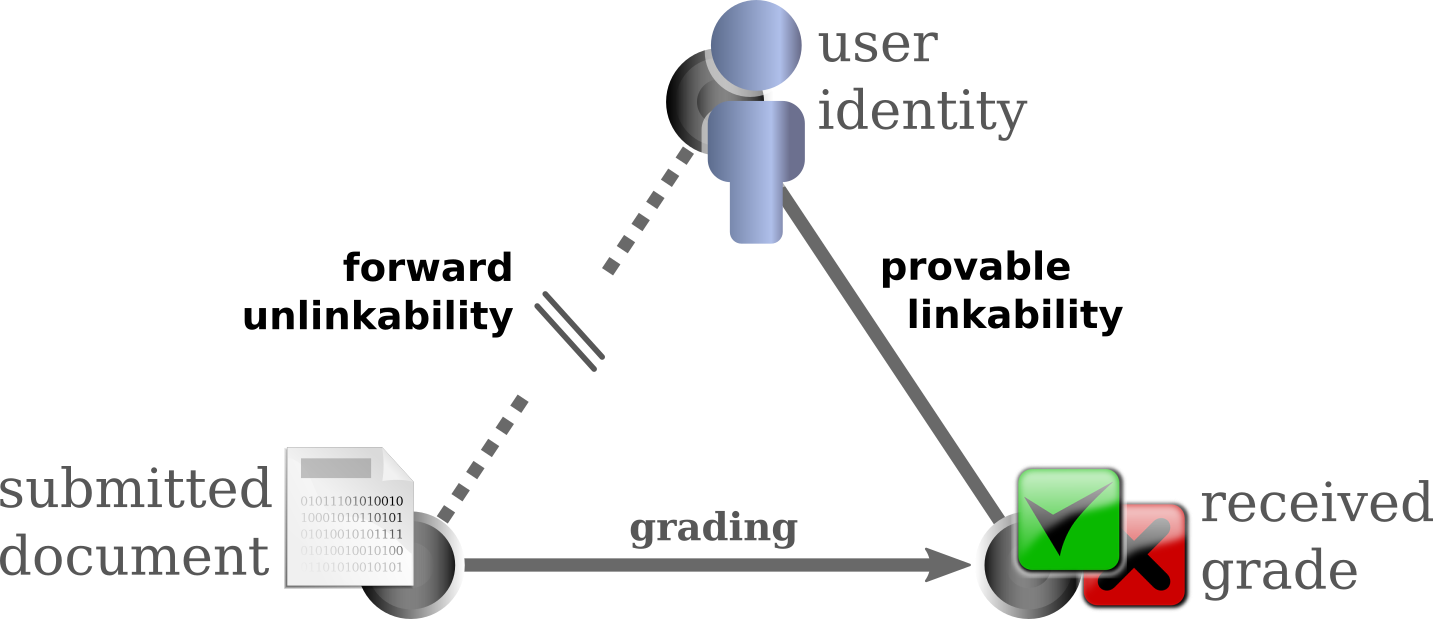
\includegraphics[width=0.88\textwidth]{images/document-submission-system/user-grade-document.png}
   \caption{Overview of system entities, their relations and desired properties.}
   \label{figure:document-submission-system:user-grade-document}
\end{figure}


Using the cryptographic technique of blind signatures
\cite{chaum_blind_1982}, we propose a protocol for this use case: a
privacy-preserving document submission and grading system that allows
students to submit documents anonymously without compromising the
correctness of the grade assignment process. 

%that guarantees perfect forward unlinkability of submitted documents and
%user identities for the students while at the same time provides a
%reliable linking of student identities to grades based on a blind
%grading process of the submitted documents.

After presenting related work in \Cref{section:document-submission-system:related-work}, we formulate a
system model and desired properties for the system in
\Cref{section:document-submission-system:anonymous-document-submission-system}. In
\Cref{section:document-submission-system:design-implementation} we suggest a protocol design that meets
these requirements, and evaluate the proposed protocol, discussing its
privacy and security properties in \Cref{section:document-submission-system:evaluation}. Furthermore,
we show the practical feasibility of the proposed solution by having
implemented a proof-of-concept prototype of the protocol, briefly
described in the same section.
    
%% contributions:
%\begin{itemize}
%
%    \item We describe a practical use case for applying blind signature
%        schemes to improve user privacy.
%
%    \item We design a protocol for a
%        document submission and grading system that guarantees perfect forward
%        unlinkability of submitted documents and user identities
%        while at the same time provides a reliable linking of
%        student identities to grades based on a blind grading
%        process of the submitted documents. 
%
%    \item We show the practical feasibility of the proposed solution by
%        implementing a proof-of-concept prototype of the protocol.
%
%    \item We evaluate the proposed protocol, discussing its privacy and
%        security guarantees and limitations.
%
%\end{itemize}


\section{Related Work}
    \label{section:document-submission-system:related-work}
%Anonymity and unlinkability are popular capabilities addressed in current literature 
%for similar problems. The former commonly resolved with the aid of onion routing 
%implementations \cite{dingledine_tor_2004}, while the latter has seen different solutions, 
%\eg blind digital signatures schemes \cite{chaum_blind_1982}.

Blind signatures schemes are widely used to
enhance the privacy of protocols by providing unlinkability. Examples 
of their use include identity management in federated login systems, \eg PseudoID 
\cite{DeyW10}, a project to protect the login data from the identity providers by 
means of blind digital signatures, 
or electronic payment systems, \eg \acs{taler} \cite{inria15}, a digital currency approach 
close to Bitcoin with the additional benefit of governmental tax traceability
without losing anonymity as blind signatures provide unlinkability to the transactions 
between customers and merchants but not between government and merchants. 
Secure voting schemes are another application area of blind signatures, 
\eg CryptoBallot \cite{Hayes13}, a cryptographically secure online voting system 
where ballots cannot be traced back to the voter as they are blinded but their counting 
and the voter identities are publicly auditable. Even though these
schemes have similarities with our problem, they would be unnecessarily
complex to adapt for the use case of document submission and grading.
%
%Smart-card technologies have been used to store credentials for identity management. 
Attribute-based anonymous credentials can be used for similar purposes,
such as in an anonymous course evaluation system for universities
\cite{StamatiouBGKLPT15}. The use-case of this project differs, however,
from our problem statement, having a focus on smart-card based anonymous
course attendance verification, introducing complexity not needed in our
scenario.
%
%The project \Ac{irma} aims at attribute-based identity 
%management in a privacy-preserving manner by storing the credentials in the smart-card 
%though these are not anonymous \cite{AlparH13}.
%
Whistleblower platforms, \eg SecureDrop \cite{fpf13} or
GlobaLeaks \cite{Hermes11}, allow a sender to submit documents
anonymously to a receiver, such as a media organization. These systems
employ anonymous and confidential communication and meta-data footprint
minimization to increase the anonymity of the sender. While maximizing
the sender anonymity, they lack, however, the provable linkability
of feedback (grades in our scenario) to identifiers, that is required in
our use case.

%
%To the best of our knowledge there is no anonymous, privacy-preserving
%system or platform allowing the submission of documents and grading with
%the functionality and properties we require, of applicability in our
%considered context.



% \section{\Acl*{adss}}
\section{Anonymous Document Submission System}
    \label{section:document-submission-system:anonymous-document-submission-system}

We aim to design a document submission and grading system, 
%that allows
%students to submit documents anonymously and at the same time to
%claim the grade they got for their submitted work. 
%
% system model
%\subsection{System Model and Assumptions}
where each student can submit a document to the system before a public
deadline. After the deadline passed, the teacher %\footnote{Without loss of generality, we assume that there is only one teacher.} 
grades all submitted
documents with either pass or fail. When all documents are graded, each
student receives the grade that the teacher assigned to the document
that was submitted by the student.

% assumptions
%\subsection{Assumptions}
We assume that students can store credentials they receive in a secure
way, do not pass them on to others and that they can communicate with
the system in a mutually authenticated and confidential way (\eg via a TLS
secured web login), and at other times in an anonymous and confidential 
way (\eg by using TLS over \acs{tor}\cite{dingledine_tor_2004}).
We assume that they are careful to include no identifying information in
the documents and that authorship attribution by stylometry is not
feasible for the adversary.
When discussing the security and reliability of the system from the
teacher's perspective, we assume that the server cannot be compromised
and that the teacher can handle secret keys in a secure way.
Furthermore, protection against ghost writing is out of scope of this
work, so we assume that students will not ask someone else to write
their documents, which reflects a general limitation for home
assignments that are allowed to be worked on outside a
teacher-controlled environment.
%
% required properties
%\subsection{Required Properties}
To achieve anonymity and correctness, we want the system to have the
following two properties:
	
\begin{propertydef}[student--document forward unlinkability]
A document cannot be linked to a student by anyone else than the
student who submitted the document, and the unlinkability remains
even after grades have been assigned to students.
\end{propertydef}
\vspace{-1em}
\begin{propertydef}[student--grade provable linkability]
If and only if a document was graded with a certain grade, the
student who submitted the document can prove that she received
this grade.
% note that these are two directions, left to right: all passed students can prove (completeness), right to left: only passed students can prove (soundness)
\end{propertydef}

%threat model
%\subsection{Threat Model}
We want our system to both protect the student's privacy and to protect
the teacher from dishonest students. Therefore we consider two different
adversaries. 
%
The first adversary tries to break the student's anonymity and is
capable of compromising any involved party except for the student
herself. In particularly it can control the teacher, the server and any
other student. Furthermore, we assume this adversary to be capable to
passively intercept all network traffic and actively inject messages. 
%The only restriction is, that this adversary must not be able to observe
%the network traffic of the anonymous channel when it is originating from
%the student's device, as otherwise end-to-end traffic correlation
%attacks against practical anonymous communication tools such as \Ac{tor}
%will become possible.
%
The second adversary tries to break the correctness of the grade
assignment and is used when discussing the security and reliability of
the system from the teacher's perspective. 
This adversary is assumed to be able to compromise one student, to
passively observe all network traffic and to actively inject messages.


\section{Protocol Design}
    \label{section:document-submission-system:design-implementation}
We implement the protocol that has the desired properties using a blind
signature scheme as described in \cite{chaum_blind_1982}, that provides the functions $blind, unblind, sign$ and
$verify$, with the property that blinding perfectly hides the data, but
signatures on blinded data can still be verified after unblinding
(informally: $unblind(sign(blind(x))) = sign(x)$).
%
\Cref{figure:document-submission-system:sequencediagram} shows the sequence of steps in our proposed protocol.
%
\begin{figure}[p]%[!ht]
    \centering
	\renewcommand{\msckeyword}{}
	\scriptsize
	\begin{msc}{}
		\setlength{\labeldist}{3ex}
		\drawframe{no}
		\declinst{student}{\parbox{3cm}{document $D$, teacher's \\public keys: $e_{pass},e_{fail}$}}{student}
		\declinst{server}{}{server}
		\declinst{teacher}{private keys: $d_{pass},d_{fail}$}{teacher}
		\setlength{\labeldist}{1ex}

		\action*{\parbox{5cm}{
			generate random $rID$ for each student
		%\\	store mappig of $rID$ to student-identifier
		}}{server}
		\nextlevel[3]

		\mess{$rID$}{server}{student} 
		\mess{\parbox{3cm}{\tiny (mutually authenticated, \\encrypted channel)}}[b]{server}{student} 
		\nextlevel[1.7]

		\messarrowscale{0}
		\mess*{\tiny done distributing $rID$s to all students}[b]{envleft}{envright}
		\messarrowscale{1.2}
		\nextlevel[1]

		\action*{\parbox{5cm}{
			generate random $b_{pass}$, $b_{fail}$\\
			$bID_{pass} = blind(rID,b_{pass},e_{pass})$\\
			$bID_{fail} = blind(rID,b_{fail},e_{fail})$
		}}{student} 
		\nextlevel[4.5]

		\mess{$D,bID_{pass},bID_{fail}$}{student}{server} 
		\mess{\tiny (anonymous, encrypted channel)}[b]{student}{server} 
		\nextlevel[1.5]

		\messarrowscale{0}
		\mess*{\tiny hand-in deadline}[b]{envleft}{envright}
		\messarrowscale{1.2}
		\nextlevel[1]

		\setlength{\inlineoverlap}{22mm}
		\inlinestart{grading}{for all submitted documents}{server}{teacher}
				\nextlevel[2.5]

				\mess{$D,bID_{pass},bID_{fail}$}{server}{teacher} 
				\nextlevel[1]

				\action*{\parbox{40mm}{
					$sbID = sign(d_{pass},bID_{pass})$ or\\
					$sbID = sign(d_{fail},bID_{fail})$
				}}{teacher} 
				\nextlevel[3]

				\mess{$sbID$}{teacher}{server} 
				\nextlevel[1]
		\inlineend{grading}
		\nextlevel[1.5]

		\mess{list of all $sbID$s}{server}{student} 
		\nextlevel[1]

		\action*{\parbox{50mm}{
						$sID = unblind(sbID,b_{pass},e_{pass})$ or\\
						$sID = unblind(sbID,b_{fail},e_{fail})$ 
		}}{student}
		\nextlevel[3.5]

		\mess{$rID, sID$}{student}{server} 
		\nextlevel[1]

		\action*{\parbox{50mm}{
						check if $sID == sign(d_{pass},rID)$\\
						or $sID == sign(d_{fail},rID)$.\\
						Register grade for student with $rID$.
		}}{server}
		\nextlevel[3.5]

	\end{msc}

	\caption{Protocol realizing an anonymous document submission and grading system.} 
	\label{figure:document-submission-system:sequencediagram}
\end{figure}%
%
First, the system server provides each registered student in the course
with a unique, random, one-time identifier $rID$ and stores the relation
of student identifiers to $rID$s for later use.
%timing attack!: distribution has to be completed before first submission!
%cutting%Distributing the $rID$s instead of using public, permanent student
%identifiers such as e-mail addresses or social insurance numbers
%avoids impersonation and replay attacks.  
Next, the student blinds the $rID$ for both the pass verification key
$e_{pass}$ and the fail verification key $e_{fail}$, using two private,
random blinding factors $b_{pass}$ and $b_{fail}$, and sends the
resulting $bID_{pass} = blind(rID,b_{pass},e_{pass})$ and $bID_{fail} =
blind(rID,b_{fail},e_{fail})$ together with $D$, the document to submit,
to the server over an anonymous, encrypted channel. %, \eg by using TLS over Tor.
%crypto attack!: we need to use two different blinding factors b if we blind the same rID for two different public keys! Otherwise the server can construct two public keys epass and efail with same modulus n and for which it holds that epass-efail=1, then the server can divide the two blinded ids and by this obtain b, because bID_pass / bID_fail = (b^epass * rID) / (b^efail * rID) = b^(epass-efail)
At this point, the server does not learn who submitted the document
because the blinding hides the $rID$, using the anonymous channel
obfuscates the network address origin and the document $D$ is assumed
to not contain any identifying information about the student.
%timing attack!: students should use home network, not university network to avoid Tor entry-exit-node correlation attacks! [as pointed out by Tobias]
After the deadline has passed, the teacher grades all submitted documents.
If a document is graded as passed, the
blinded identifier $bID_{pass}$ that was submitted together with the document
is signed with the private pass signing key $d_{pass}$ of the teacher. If the grade is fail, $bID_{fail}$
will be signed with the teacher's private fail signing key $d_{fail}$.
When all documents are graded, the server publishes a list of all signed
blinded identifiers. 
The student fetches the list, picks the signed blinded identifier that
belongs to her and unblinds it. 
The student will try both public verification keys $e_{pass}$ and $e_{fail}$
to check which grade she received. 
%She will also need to try all signed blinded identifiers in the list from the server, as they do not contain identifying information, but the protocol could easily be extended to have a student-chose pseudonym attached to both the submission and the list (eg a hash of $D$).
By this, the student obtains a signed identifier $sID = sign(rID)$
that proves that she received the grade corresponding to
the signing-key.
Finally, she sends $sID$ to the server, the server checks the signature,
looks up the student identifier that belongs to $rID$, and registers the
corresponding grade for the student, not learning which document the
student submitted.

%\subsection{Other Grading Scales and Submission Acknowledgements}
%
%The basic protocol as outlined above can be extended in different ways
%to incorporate more features and functionality. 
%
%The grading scale can easily be extended to any discrete scale, \eg an
%A-F scale instead of the pass/fail scale considered so far, by
%introducing more grade keys. Instead of having only the
%$e_{pass},d_{pass}$ and $e_{fail},d_{fail}$ keypairs, the teacher would
%generate and publish one keypair per grade, use them accordingly during
%grading and the students would check the signed blinded results against
%all of them. This comes, however, with the disadvantage of smaller
%anonymity sets as they depend on the number of other students that
%received the same grade, as discussed later in the evaluation.
%
%Another useful functionality is the acknowledgement of submissions by
%the server, so that in the case of a technical failure that causes a
%document not to be graded, the student still has a mean to prove that
%she handed in a document before the deadline. A straightforward implementation
%of this would be that the server signs each submitted document immediately
%with an extra key for that purpose, a ``handed-in key''. If later the
%student discovers that there is no entry for her in the result list,
%she can choose to give up her anonymity and present the signed document
%to the server, proving that she handed it in before the deadline.
%
%%oldTODO: extension: submission acknowledgement (simple solution: server returns signature (with extra hand-in key) on D upon submission, drawback: student has to give up anonymity for claiming it (maybe do another round of grading without giving up anonymity by only accepting signed documents for this second round, but what if result still incomplete after this round? maybe there's some cool zero-knowledge proof based solution for that, or secure mixing based solution would solve that?)
%
%% acknowledgement solution: by signing with a handed-in-key, but 
%% have to be thought through more, because students can cheat by presenting the 
%% acknowledgement and not claiming their grade
%
%%oldTODO: another extension: multiple grades (or in evaluation?)

\section{Discussion and Evaluation}
    \label{section:document-submission-system:evaluation}
%TODO: fix same-blinding-factor-deanonymization attack in implementation!
We have implemented a proof-of-concept prototype (see \url{http://www.ter.se/dss/}) %\footnote{The code of the prototype is available at http://www.ter.se/dss/}, 
which is a collection of C programs 
for the various operations performed by the student, server and teacher, realizing 
the described protocol. The prototype uses the free cryptographic library \texttt{Libgcrypt} \cite{fsf07}. 
% negligible performance issues, even on constraint devices
%
In the following, we do an informal security and privacy evaluation,
discussing why the previously defined properties hold and various
attacks will not succeed. We do not cover implementation-based attacks
though, such as cross-site-scripting attacks on a web-interface.

\paragraph{Student--document forward unlinkability}
%forward unlinkability: only k-anonymity among the other students with the same grade
The student identity is directly linked to the random identifier $rID$. 
But when submitting the document $D$, the $rID$ is perfectly hidden by the
random blinding factors known only to the student.
We assume that there is no identifying information contained in the
document, so after submission the server cannot link
student identifiers to documents.
To achieve forward unlinkability, this has to hold even after the grades
have been assigned to students.  
During grading, documents are linked to grades, which is a binary domain in our
case. The grade information is attached to the blinded $rID$ in form of 
a signature with one out of two keys, that can be transformed in a verifiable
signature on the unblinded $rID$ only by the student. The properties of the
blind signature scheme provide the unlinkability between this unblinded
signature and the blinded data that was submitted together with the document.
At the same time, the signature is provided to the server together with the $rID$ 
when the students claim their grades, so they provide an unambiguous
mapping from every $rID$ to a grade. As a consequence, we do not get
perfect unlinkability of student identifiers and documents, but only
\emph{k-anonymity}, where $k$ is the number of students who received the same
grade. This is a general limitation of every system where the grading
party is not trusted and the assignment of grades to student identifiers 
is verifiable. A worst-case example is a situation
where only one student received the grade ``fail'', so the
teacher can infer that the only document she graded with ``fail''
must belong to this student.
Another limitation is the fact, that the anonymity for all students with
a certain grade is reduced whenever one student with the same grade
gives up their anonymity voluntarily or becomes compromised by the
adversary.


\paragraph{Student--grade provable linkability}
% two directions
The provable linkability of student identifiers to grades has two
directions: (a) soundness: if a student can prove that she received a certain
grade, then she must have submitted a document that was graded
accordingly, and (b) completeness: if a document submitted by a student was graded
with a certain grade, then the student can prove that she received that
grade. 
%
We show (a) by contrapositive, so we assume that the student did not
submit a document that was graded with the grade that the student
claims. Now we see that the student cannot prove that she received
that grade: she cannot present a valid signature on the $rID$
assigned to her, made with the private key corresponding to the grade,
because the private signing key was used by the teacher only to sign
other blinded $rID$s that were submitted together with documents that
were graded accordingly.
%
For (b) we see directly that if a submitted document was graded with a
certain grade, the teacher put a signature on the blinded $rID$
submitted together with the document and publishes that later on. So the
student can derive a valid signature on her $rID$ by unblinding the
published information and therefore can prove to anyone knowing the
public verification key, that she received that grade.


\paragraph{Timing and Correlation Attacks}
% importance of deadlines (after rID handout, hand-in deadline/bulk-download of result)
To avoid timing attacks, it is important that certain events in the
protocol do not happen before others. For example, the hand-in of
documents must not start before all students received their $rID$s
(denoted by the first dashed line in the message sequence chart in
\Cref{figure:document-submission-system:sequencediagram}), otherwise the anonymity set for the
submitting students is immediately reduced to those who already received
their $rID$. 
For a similar reason it is important that the server publishes the
result list with the signed, blinded $rID$s after the hand-in deadline
and as a complete list. The latter is important, because if students for
example would request their individual entries without downloading the
complete list, the server could correlate these requests for specific
entries (that the server can link to documents) with requests for
registering a grade (which contain the identifier $rID$), that might
happen shortly after each other.
%
% Tor end-to-end traffic correlation attack (Tobias' comment)
End-to-end traffic correlation attacks are also relevant for the concrete
implementation of the anonymous channel. \acs{tor}, for example, does not
protect against an adversary that can observe both traffic going into
the \acs{tor} network and traffic coming out of it \cite{dingledine_tor_2004},
so the students should for example be advised not to use the university
network when submitting their documents, because it is likely that the
same party operates both the university network and the system server
and therefore could observe both ends of the students' connections.


\paragraph{Impersonation and Replay Attacks}
%importance of using $rID$ and not a public student id
To avoid impersonation and replay attacks, it is important not to use a
public or permanent student identifier such as the students' e-mail
addresses. Otherwise, an attacker could
impersonate a student, \eg to damage her reputation by submitting
a low-quality document in her name. Therefore, we use the 
unique, random, one-time identifier $rID$ and distribute it over a
mutually authenticated and encrypted channel to the student. This makes 
impersonation without the cooperation of the student impossible because
the attacker does not know which $rID$ was assigned to a 
student. It also prevents replay attacks,
as the $rID$ binds the messages both to the student and to the 
current course, because even if the same protocol is used for several
courses, the same student will receive a new $rID$
in each new protocol run.

\paragraph{Attacks on Combined Cryptographic Primitives}
% won't discuss them really but refer to papers (double-check attacks on RSA paper)
% discuss shared-blinding-factor attack
Attacks on the used cryptographic primitives, such as public key
cryptography, hash functions and blind signatures, are out
of scope of this work, so we assume them to be secure. However, we have
to be careful to use these tools in a secure way, especially when
combining them with each other. It is, for example, important to use two
different blinding factors $b_{pass}$ and $b_{false}$ when blinding the
$rID$.  Otherwise, if for ease of implementation one would use only one
common blinding factor $b$ for both blindings, the server would be able
to mount the following de-anonymization attack: 
%
\newcommand{\modn}{\ensuremath{\quad(\mathrm{mod}\ N)}}
The server generates specially prepared public keys $e_{pass} = \langle
N,e \rangle$ and $e_{fail} = \langle N,e' \rangle$ with the property
that both share the same modulus $N$ and the public exponents have a
difference of one: $e - e' = 1 \modn$.
%For example generating e_pass normally and then setting e_fail =
%(e_pass-1,n). The latter will be an invalid public key (in the sense
%that the DSS does not have a corresponding private key to it), but as
%long as the student does not check for these properties the attack works.
If the student blinds her $rID$ for these keys using a common blinding
factor $b$, she will submit the following two values to the server:
$bID_{pass} = blind(rID,b,e_{pass}) = rID \cdot b^{e} \modn$,
$bID_{fail} = blind(rID,b,e_{fail}) = rID \cdot b^{e'} \modn$.
Now, the server can simply divide the two values to obtain the blinding
factor $b$:
$bID_{pass} / bID_{fail} = (b^{e}\cdot rID) / (b^{e'}\cdot rID) =
b^{e-e'} = b \modn$.
Having learned $b$, the server can unblind the $bID$s and obtain $rID$,
thus having de-anonymized the student.



%\paragraph{System Implementation Attacks}
%Attacks on the used system components are also out of scope of this work.
%So we simply assume that there are no web-security flaws that allow for
%common attacks such as cross-site-scripting or
%cross-site-request-forgery on the server side interface, that injection attacks on
%the server's database are prevented, that secure
%versions of TLS are used for the authenticated channels and the involved
%certificate authorities are not compromised, that \Ac{tor} is used in a secure
%way to avoid side-channels attacks such as browser fingerprinting, that
%students use secure devices to prevent leakage of their credentials and
%that the system usability facilitates a secure usage.
%Even though these threats are out of scope of this work, they are
%important in practice and have to be taken into account when
%implementing an actual system.


\section{Conclusions and Limitations}
    \label{section:document-submission-system:conclusions-future-work}
%Blind signature schemes are a standard cryptographic technique used for example
%in digital currencies or voting schemes, where a user signs a message without
%being able to know the content of the message.

We have described a practical application for blind signatures schemes in the context 
of a document submission and grading system to 
improve the privacy of students without undermining the correctness 
of the grading process.
%
%We formulated two main required properties,
%student--document forward unlinkability (to protect the students' privacy even after the 
%grading process) and student--grade provable linkability (to guarantee that a certain 
%grade can only be claimed by a student who submitted a document with such grade),
%and designed a protocol that guarantees these properties.
%
%Our protocol specification has been implemented in a proof-of concept
%prototype using the standard cryptographic library \texttt{Libgcrypt},
%and we carried out a security and privacy evaluation of the protocol
%showing how the defined properties hold. We also analysed how different
%types of attacks, such as timing, correlation, impersonation and replay
%attacks are prevented. Moreover, we discussed the importance of careful
%protocol design when combining cryptographic primitives by providing an
%example for a seemingly innocent implementation simplification that
%actually introduces a vulnerability for a complete de-anonymization
%attack.
%
We found that it is feasible to implement such a
system, qualified
only by the limitations derived from the scenario, \eg that the provided
$k$-anonymity depends on the number of other students who received the
same grade, that students can choose not to reveal their grade, and that
documents cannot be linked to students even where this might be desired
for pedagogical reasons or penalty measures for plagiarism
that go beyond grading the work with fail.
%

The basic protocol described here can be extended with more
functionality such as having several teachers do the grading, using more
fine grained grading scales (with the limitation that this decreases the
anonymity sets), issuing submission acknowledgements or including
individual feedback without breaking the anonymity properties.

%future work
%For future work we want to look at the trade-off of anonymity and
%accountability, for example systems with a limited trusted third party,
%so that documents can be linked to identifiers in case of plagiarism or
%other disputes. Furthermore, we plan to explore the applicability of
%anonymous attribute-based credentials to enrich the functionality of the
%system, for example to include anonymous credentials for having met
%prerequisites of a course.
%A formal proof of the security and privacy aspects of our protocol is
%another goal of future work that would provide stronger guarantees
%compared to the privacy and security evaluation conducted in this paper.
%Finally, we aim for developing a secure and usable application from the
%prototype that can be used in practice for a university course.

% nice-to-have: Find Ian Goldberg's reference for delay idea (to mitigate network monitoring) [also read up on different solutions for this same problem: Mixmaster and Mixminion, referenced in https://blog.torproject.org/blog/traffic-correlation-using-netflows ]


\section*{Acknowledgments}
    \label{section:document-submission-system:acknowledgments}
This research has been funded by the \Acl{ssf} grant SSF FFL09-0086 and the \Acl{vr} 
grant VR 2009-3793.


%%%%%%%%%%%%%%%%%%%%%%%%%%%%%%%%%%%%%%%%%%%%%%%%%%%%%%%%%%%%%%%%%%%%%%%%%%%%%%%
%In the bibliography, use \texttt{\textbackslash textsuperscript} for ``st'', ``nd'', ...:
%E.g., \enquote{The 2\textsuperscript{nd} conference on examples}.

% \bibliographystyle{utils/splncs03}
% \bibliography{ppsds}

%%%%%%%%%%%%%%%%%%%%%%%%%%%%%%%%%%%%%%%%%%%%%%%%%%%%%%%%%%%%%%%%%%%%%%%%%%%%%%%

% \end{document}